\section{Analysis}
Our two basic research questions were addressed individually.

\subsection{Question 1}
Technically, the data we collected were asymmetric; that is, we have separate data from when group $A$ serves as the target and group $B$ serves as the distracter than when group $A$ serves as the distracter and group $B$ serves as the target. See Figure~\ref{fullacc} for the non-symmetric accuracies. McNemar's test failed standard tests of significance $p > 0.1$, so we decided to pool the data. 

To answer our first question, we did a simple binomial t-tests comparing participants' actual performance to chance ($\pi=0.5$). Using this paradigm, we found that $135/136$ tests were significant at the $p<0.05$ level; the last test was still significant at the $p<0.10$ level. While there was clear variation in these probabilities, it seems clear that in general, people were able to distinguish among them better than chance. 

The most difficult pair for participants to distinguish between were “p4m” and “pmm” (see Figure~\ref{pmmp4m} for an example). Interestingly, an expert given a small amount of time should have almost no trouble distinguishing them, as the lack of 4-fold rotation is quite obvious in "pmm." Across the 96 participants, only 56.8\% of trials were successful. For comparison, the average accuracy among all trials was 76.8\%. However, there remains a possibility that certain groups are nearly indistinguishable to non-experts.

\begin{figure}[!ht]
\centering
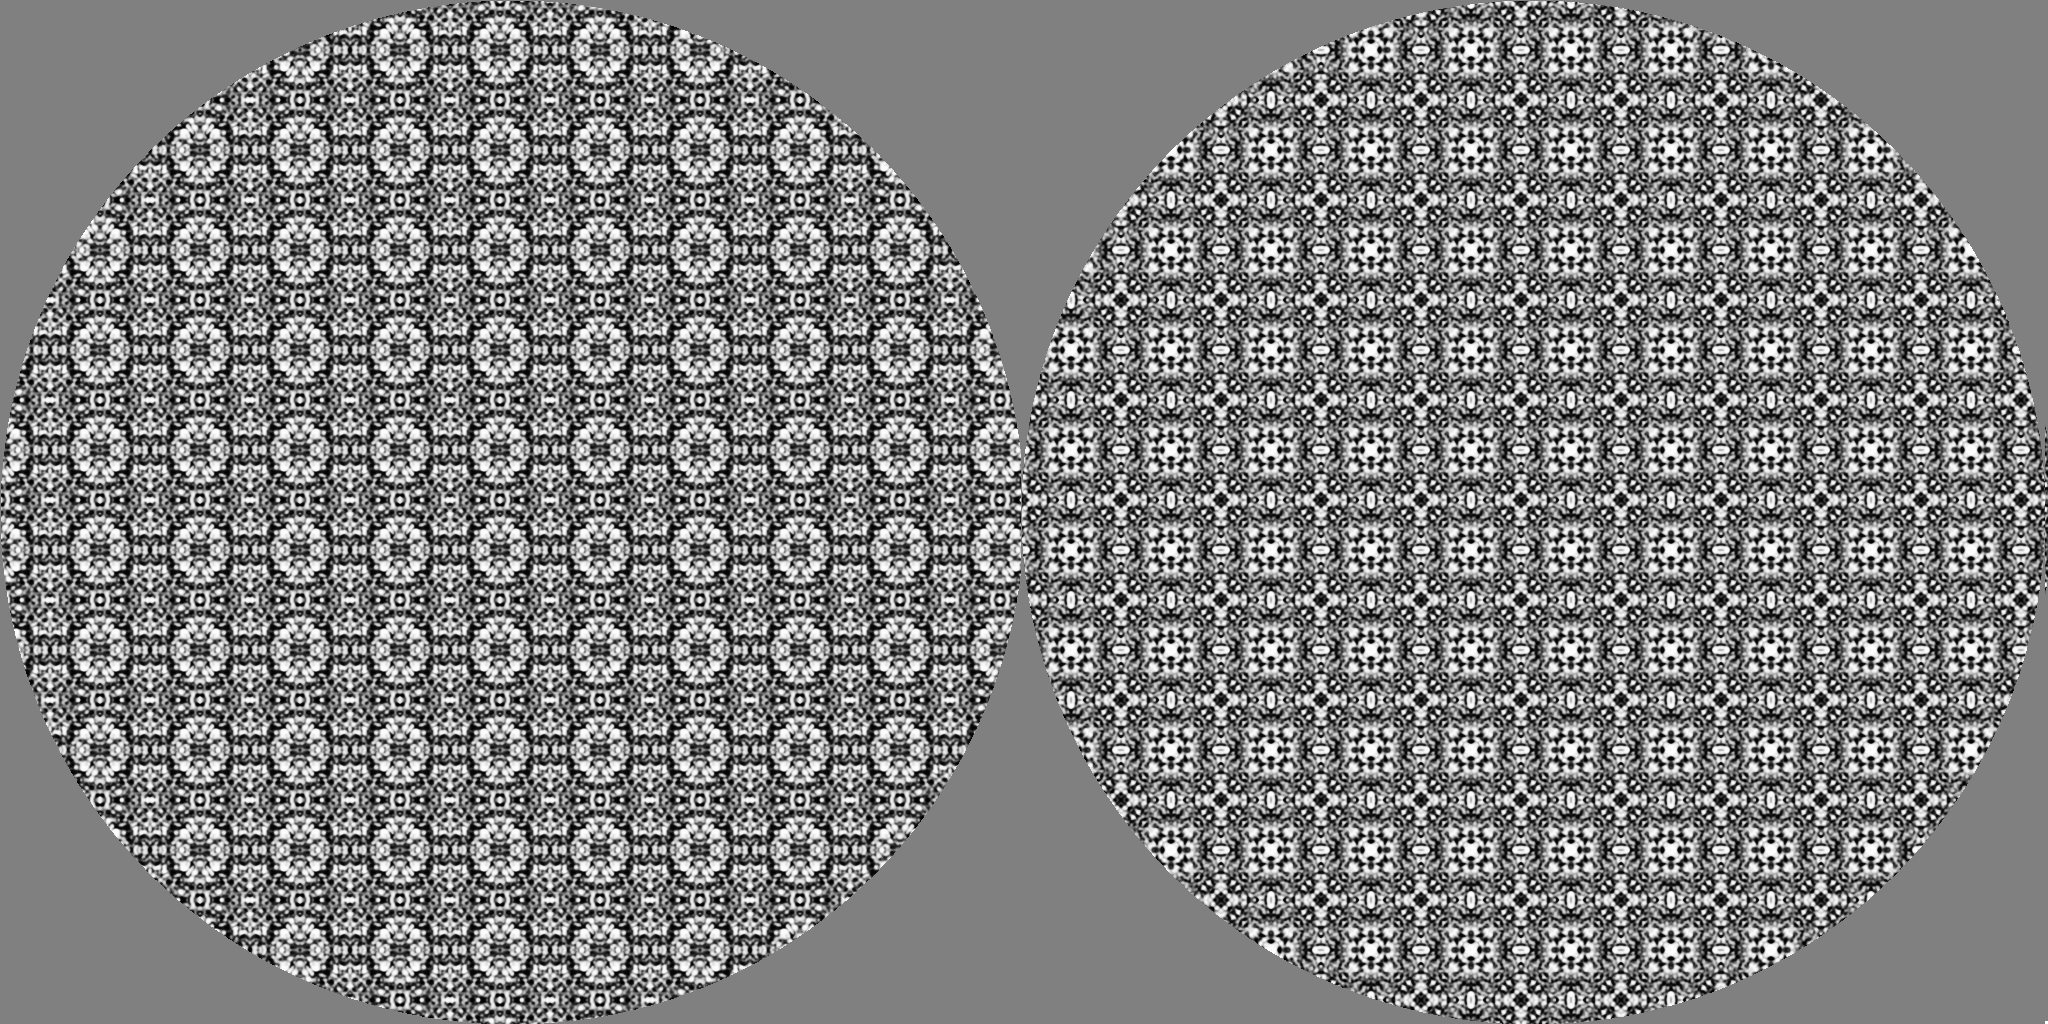
\includegraphics[width=0.9\columnwidth]{pmmp4m}
\label{pmmp4m}
\caption{PMM on the left (note the tiles lack reflection on the horizontal axis, but have it on the vertical axis), P4M on the right}
\end{figure}

\begin{figure}[!ht]
\centering
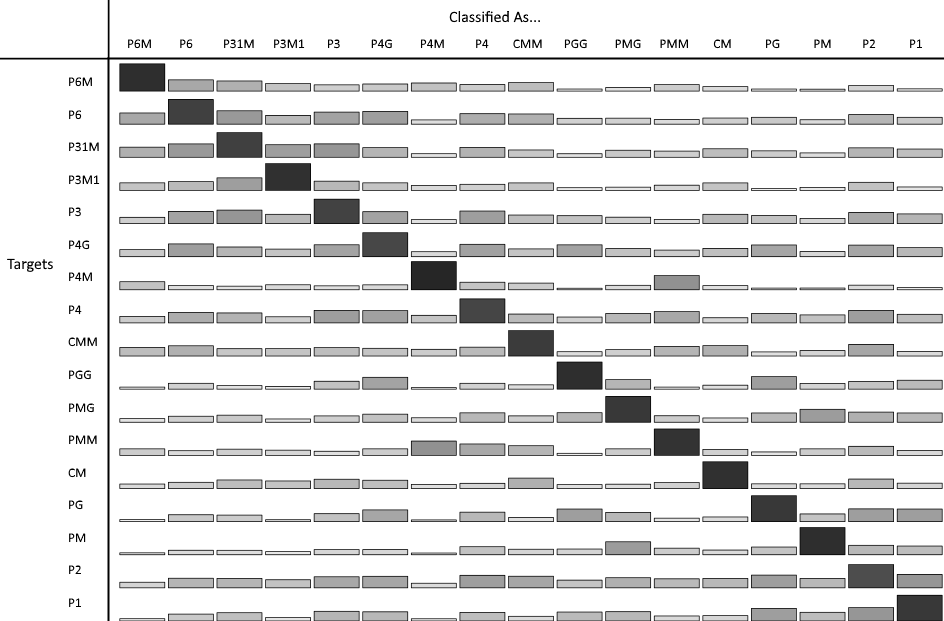
\includegraphics[width=0.9\columnwidth]{accuracies-grayscale}
\label{fullacc}
\caption{On the vertical we have the targets. On the top are the distracters. Main diagonal represents the aggregate accuracy in labeling that group correctly. The darker the bar, the closer to 1.0.}
\end{figure}

\subsection{Question 2}
To answer our second question, we used a Linear Mixed Effects Regression (GLMM) model. We tried to determine which symmetries contributed to accuracy. Thus, we used a comparison of each task's symmetries as the model.
\begin{enumerate}
\item 2-Fold Rotation, 3-Fold Rotation, 4-Fold Rotation, 6-Fold Rotation (True, False). In this case, groups with 6-Fold are guaranteed to have 3-Fold and 2-Fold.
\item Reflection, Glide Reflection, or nothing along the four main axes ($T_1, T_2, D_1, D_2$)
\item Tile Shape. This feature is not included in the group-theoretic analysis, but might play a role
\item Subgroup distance, computed with Djikstra's algorithm. 
\end{enumerate}

We used two random effect variables: the participant and the specific task; while it would contain the same groups, the group being on the top or bottom might play some small role. While we could have iteratively designed a uniform test set avoiding this issue, random effects allow us to control for the variance our methodology caused.

\begin{figure}[!ht]
\centering
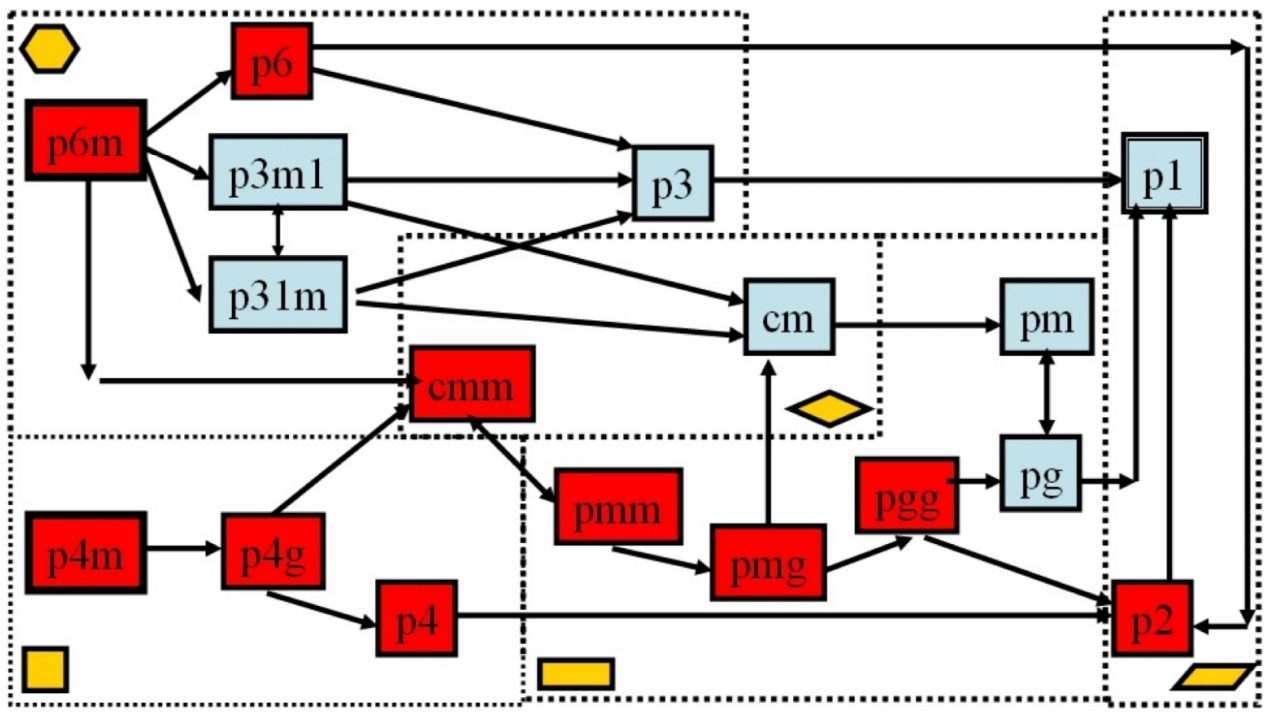
\includegraphics[width=0.9\columnwidth]{Yanxi_Graph}
\label{graph}
\caption{The subgroup relation graph}
\end{figure}

We found the best overall model by lowest AIC, from the pool of features described earlier. This model included distance, but additionally included the $T_1$ axis, which would correspond to bilateral reflection symmetry, the $D_1$ axis, which is the positive diagonal, along with 4-fold and 3-fold rotation. See Table~\ref{fixeff} for the fixed effects in a model including all possible features.